\documentclass{article}
\usepackage{graphicx}
\usepackage{amsmath}
\usepackage{booktabs}
\usepackage{hyperref}
\usepackage{geometry}

\geometry{a4paper, margin=1in}

\title{Multi-Horizon Solar Irradiance Forecasting Using a Hybrid BiLSTM-GBDT Model: A Study Across 22 BSRN Stations}
\date{\today}

\begin{document}

\maketitle

\section{Abstract}
This paper presents a comprehensive study on the generalization of a hybrid Gradient Boosting Decision Tree (GBDT) and Bidirectional Long Short-Term Memory (BiLSTM) model for medium-term solar irradiance forecasting. While hybrid architectures are established in the literature, this work distinguishes itself by rigorously evaluating model performance across a diverse dataset of 22 meteorological stations from the Baseline Surface Radiation Network (BSRN). We focus on the model's ability to generalize across varying climatic zones and environmental conditions without relying on detailed meteorological parameters or external weather predictions. Unlike traditional short-term forecasting studies, this research focuses on a medium-term horizon (72 hours), utilizing a comprehensive 2-week input window (336 hours) to capture long-range temporal dependencies. Our results demonstrate that the model effectively captures both structural and temporal patterns across different locations, offering a robust solution for solar power generation planning in data-constrained environments.

\section{Introduction}
The integration of solar photovoltaic (PV) systems into the global energy mix is accelerating, driven by the need for sustainable and renewable energy sources. However, the inherent intermittency and variability of solar irradiance pose significant challenges for grid stability and energy management. Accurate forecasting of solar irradiance is, therefore, a prerequisite for efficient dispatching, storage management, and market participation.

Forecasting techniques generally fall into three categories: physical models, statistical models, and machine learning (ML) approaches. While physical models rely on numerical weather prediction (NWP) data, statistical and ML models learn patterns directly from historical data. Recently, hybrid models that combine the strengths of different algorithms have shown superior performance.

This paper implements a hybrid model that integrates the feature extraction capabilities of LightGBM (a GBDT implementation) with the sequence modeling power of BiLSTMs. The LightGBM component acts as a sophisticated feature extractor, capturing non-linear relationships between basic variables and irradiance, while the BiLSTM component models the temporal dynamics and dependencies over time.

While the combination of GBDT and BiLSTM has been explored in previous studies, the primary contribution of this work lies in the extensive validation and generalization of this architecture across a global scale. We utilize high-quality data from 22 distinct BSRN stations, covering a wide range of climatic zones and latitudes. The novelty of this research is the assessment of the model's robustness and adaptability to different locations and environmental features, specifically demonstrating its efficacy in scenarios where detailed meteorological data (such as cloud cover, aerosol depth, or precipitable water) is unavailable. Furthermore, we target a medium-term forecast horizon of 72 hours (3 days), which presents a greater challenge than the typical 1-hour or 24-hour horizons often explored in the literature.

\section{Related Work}
\textit{[This section is left blank for comparative analysis and literature review.]}

\section{Methodology}

\subsection{Hybrid Model Architecture}
Our proposed model employs a two-stage hybrid architecture:

\begin{enumerate}
    \item \textbf{Stage 1: Feature Extraction with GBDT (LightGBM):} 
    We first train a Gradient Boosting Decision Tree (LightGBM) on the engineered features (time, lag, and meteorological variables) to predict the target variable (GHI). This model excels at capturing structural, non-linear relationships in tabular data. The predictions from this model are then added as a new feature, effectively enriching the input space for the subsequent sequence model.
    
    \item \textbf{Stage 2: Sequence Modeling with BiLSTM:}
    The enriched feature set is fed into a Bidirectional LSTM (BiLSTM) network. The BiLSTM processes the input sequence in both forward and backward directions, allowing it to capture context from both past and future states within the window.
    
    The mathematical formulation for the LSTM unit is as follows:
    \begin{align*}
        f_t &= \sigma(W_f \cdot [h_{t-1}, x_t] + b_f) \\
        i_t &= \sigma(W_i \cdot [h_{t-1}, x_t] + b_i) \\
        \tilde{C}_t &= \tanh(W_C \cdot [h_{t-1}, x_t] + b_C) \\
        C_t &= f_t * C_{t-1} + i_t * \tilde{C}_t \\
        o_t &= \sigma(W_o \cdot [h_{t-1}, x_t] + b_o) \\
        h_t &= o_t * \tanh(C_t)
    \end{align*}
    
    Our architecture consists of:
    \begin{itemize}
        \item \textbf{Input Layer}: Accepts a sequence of length $T_{in} = 336$ hours.
        \item \textbf{BiLSTM Layers}: 2 stacked layers with 128 hidden units each.
        \item \textbf{Output Layer}: A fully connected (dense) layer that projects the last hidden state to the output horizon $T_{out} = 72$ hours.
    \end{itemize}
    
    The model is trained using the Mean Squared Error (MSE) loss function and the Adam optimizer.
\end{enumerate}

\subsection{Datasets}
The study utilizes data from the Baseline Surface Radiation Network (BSRN), a project of the World Climate Research Programme (WCRP) aimed at detecting important changes in the Earth's radiation field.

\begin{itemize}
    \item \textbf{Source}: 22 meteorological stations.
    \item \textbf{Data Type}: High-resolution solar radiation data (Global Horizontal Irradiance - GHI).
    \item \textbf{Selection Criteria}: The stations were chosen to represent a diverse set of geographical locations (varying latitudes and longitudes) to ensure the model's robustness across different climatic conditions.
\end{itemize}

\subsection{Data Engineering}
The raw data underwent a rigorous preprocessing pipeline to ensure quality and compatibility with the hybrid model:

\begin{enumerate}
    \item \textbf{Cleaning and Resampling}: 
    Raw data files (`.tab` format) were parsed to extract timestamp, irradiance, and location metadata. Negative irradiance values were clamped to zero. Missing values were handled using forward-fill followed by backward-fill strategies. The data was then resampled to an hourly frequency to standardize the time steps.
    
    \item \textbf{Feature Engineering}:
    We generated a rich set of features to aid the model:
    \begin{itemize}
        \item \textbf{Cyclical Time Features}: Sine and Cosine transformations of the Hour-of-Day and Day-of-Year to preserve the cyclical nature of time.
        \item \textbf{Lag Features}: Historical GHI values at 24-hour and 168-hour (1 week) lags to capture daily and weekly seasonality.
        \item \textbf{Meteorological Features}: Temperature, Humidity, and Pressure were extracted and mapped from the raw files where available.
    \end{itemize}
    
    \item \textbf{Sequence Generation}:
    The data was transformed into sliding window sequences.
    \begin{itemize}
        \item \textbf{Input Window}: 336 hours (2 weeks) of historical data.
        \item \textbf{Output Window}: 72 hours (3 days) of future targets.
    \end{itemize}
    
    \item \textbf{Normalization}:
    All features were normalized using Min-Max Scaling to the range [0, 1] to facilitate stable convergence during neural network training.
\end{enumerate}

\subsection{Irradiation to Power Generation Process}
While the primary output of our model is Global Horizontal Irradiance (GHI), this serves as the fundamental input for estimating solar power output. The relationship between environmental factors and solar power generation is governed by the strong correlation between temperature, irradiance, and energy output (in Watts).

The process is as follows:
\begin{enumerate}
    \item \textbf{Irradiance Prediction}: The hybrid model generates the 72-hour GHI forecast.
    \item \textbf{Power Conversion}: This forecasted irradiance is used as the primary driver in a PV power conversion model. Intuitively, higher irradiance leads to higher power output, but this is modulated by temperature (PV efficiency decreases as temperature increases).
    \item \textbf{Rationale}: We decouple the irradiance forecasting from the power conversion because irradiance is the primary stochastic variable. By accurately predicting the meteorological potential (GHI), we can apply deterministic physical models (considering panel efficiency, area, and temperature coefficients) to derive the final power output. This two-step approach allows for greater flexibility in simulating different PV system configurations.
\end{enumerate}

\section{Results \& Analysis}

\subsection{Exploratory Data Analysis}
We began by analyzing the distribution and characteristics of the solar irradiance data across the 22 sites.

\begin{figure}[h]
    \centering
    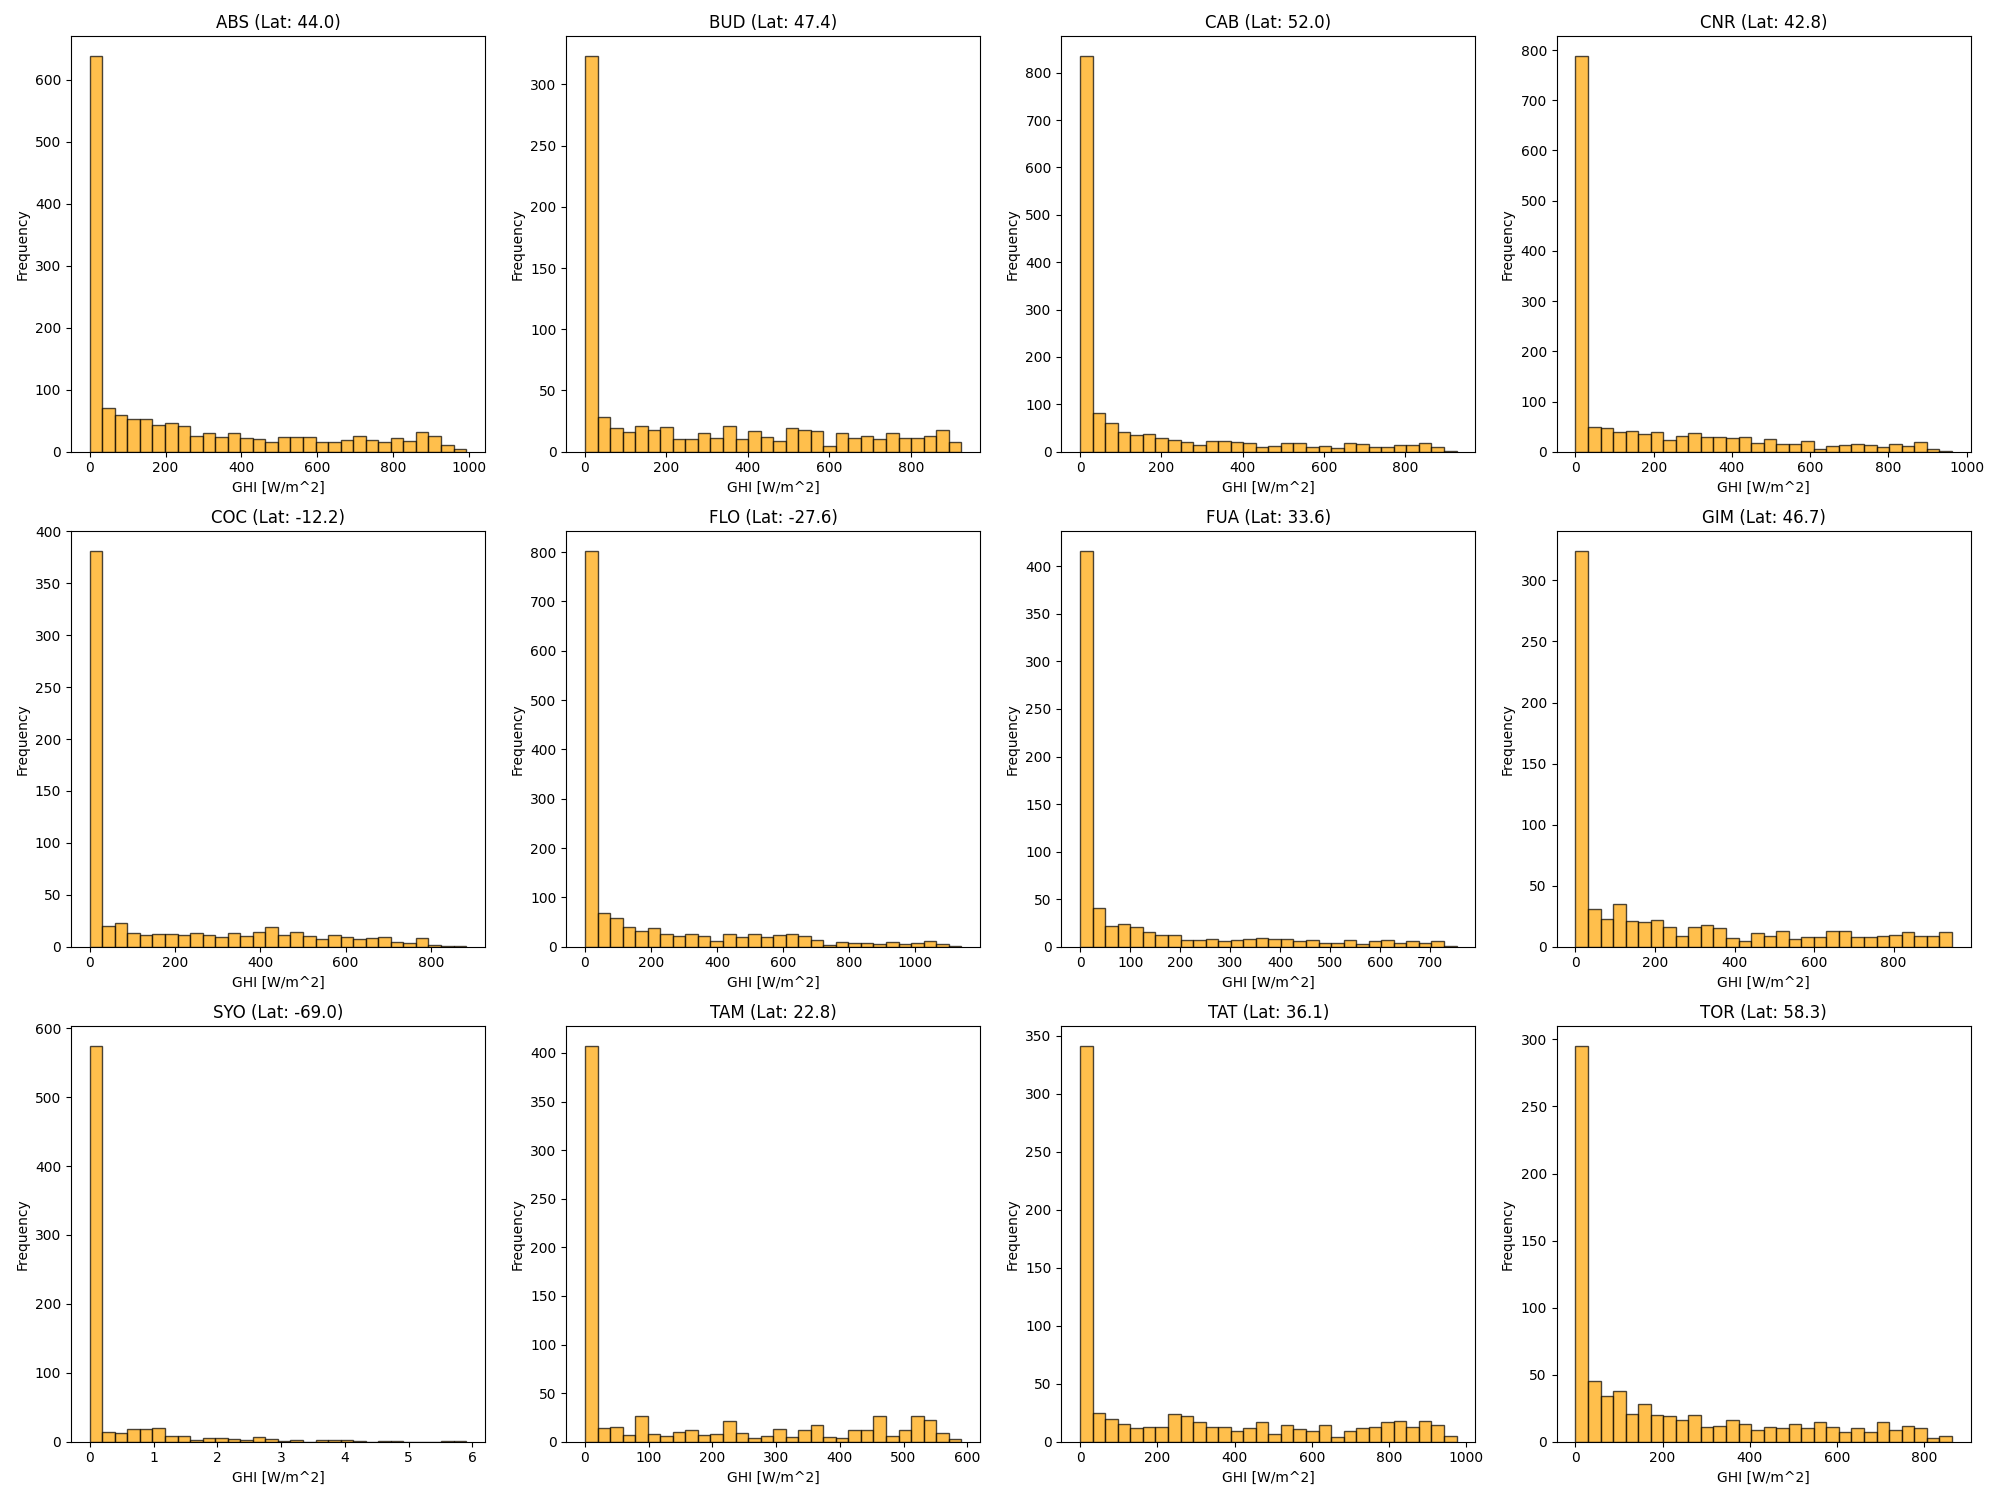
\includegraphics[width=0.9\textwidth]{artifacts/eda_ghi_distribution.png}
    \caption{Distribution of Global Horizontal Irradiance (GHI) across different sites.}
\end{figure}

The diurnal cycles for each site were also examined to understand the average daily profile.

\begin{figure}[h]
    \centering
    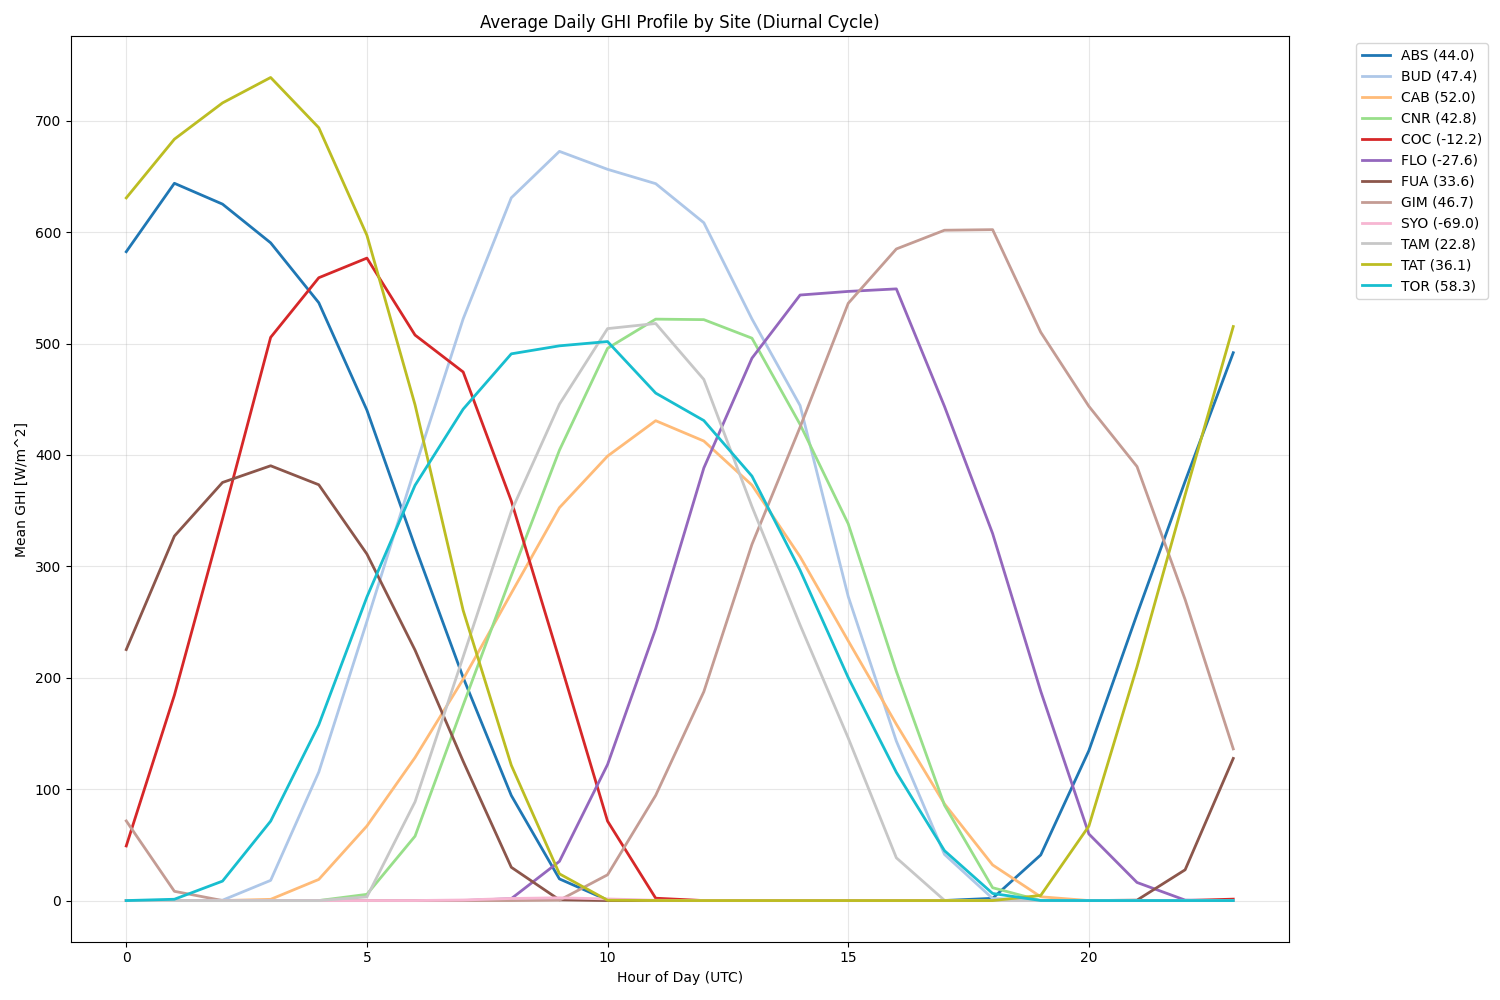
\includegraphics[width=0.8\textwidth]{artifacts/eda_diurnal_cycle.png}
    \caption{Average Daily GHI Profile (Diurnal Cycle) by Site.}
\end{figure}

Correlation analysis confirmed the strong relationship between the engineered features (particularly lags and solar geometry) and the target variable.

\begin{figure}[h]
    \centering
    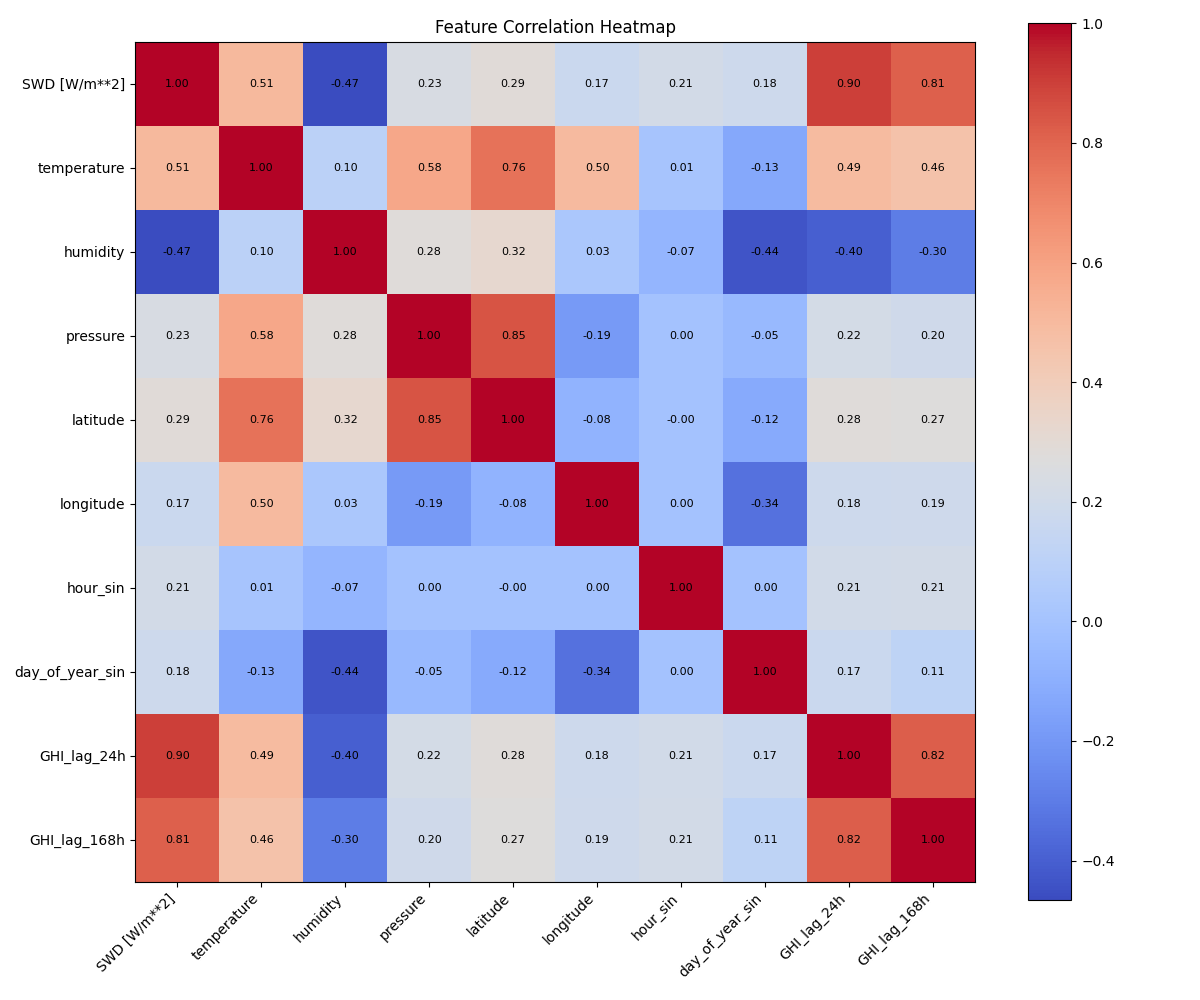
\includegraphics[width=0.7\textwidth]{artifacts/eda_correlation.png}
    \caption{Feature Correlation Heatmap.}
\end{figure}

\subsection{Model Performance}
The training process showed stable convergence, as evidenced by the loss curves.

\begin{figure}[h]
    \centering
    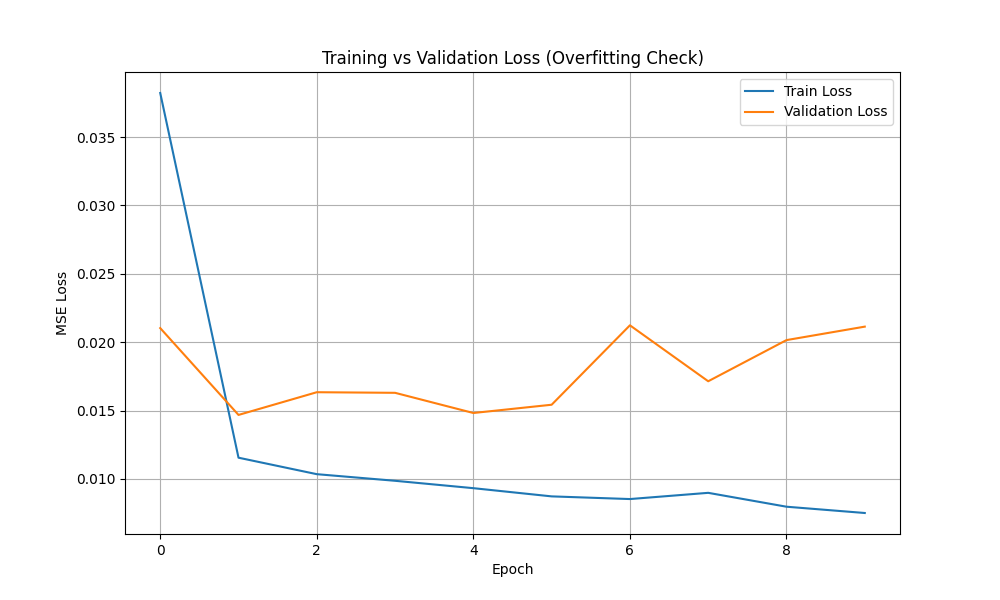
\includegraphics[width=0.7\textwidth]{artifacts/loss_curve.png}
    \caption{Training and Validation Loss Curves.}
\end{figure}

We evaluated the model on a held-out test set. The forecast samples below demonstrate the model's ability to track the diurnal pattern over the 3-day horizon.

\begin{figure}[h]
    \centering
    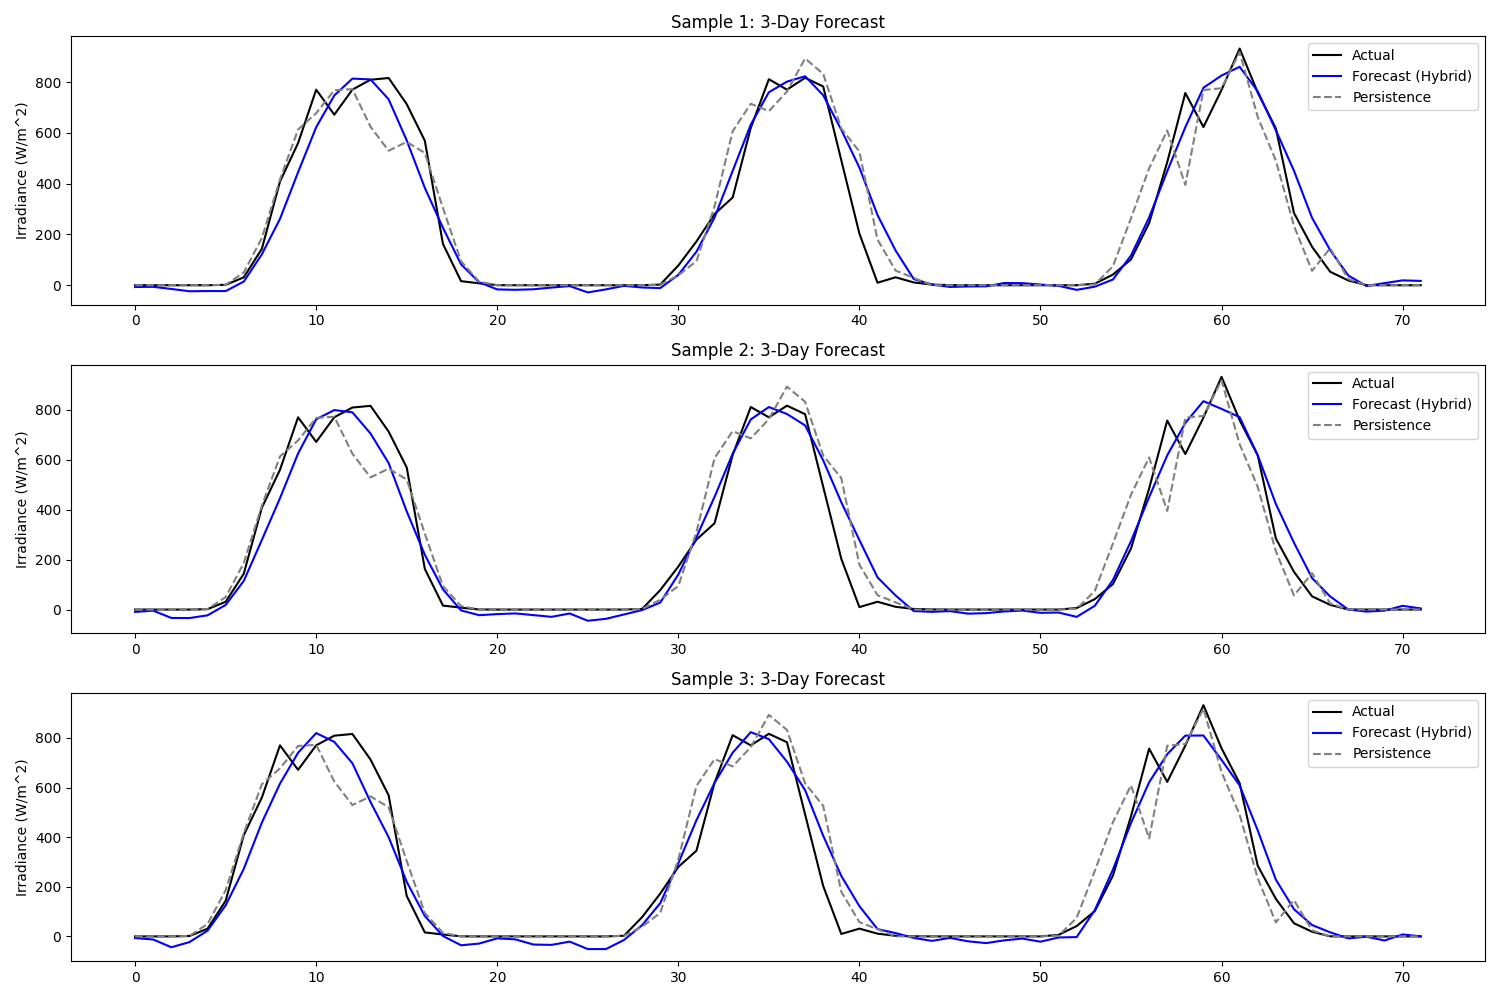
\includegraphics[width=0.9\textwidth]{artifacts/forecast_samples.png}
    \caption{Sample 3-Day Forecasts vs Actuals and Persistence Baseline.}
\end{figure}

The scatter plot of predicted vs. actual values indicates a strong alignment along the diagonal.

\begin{figure}[h]
    \centering
    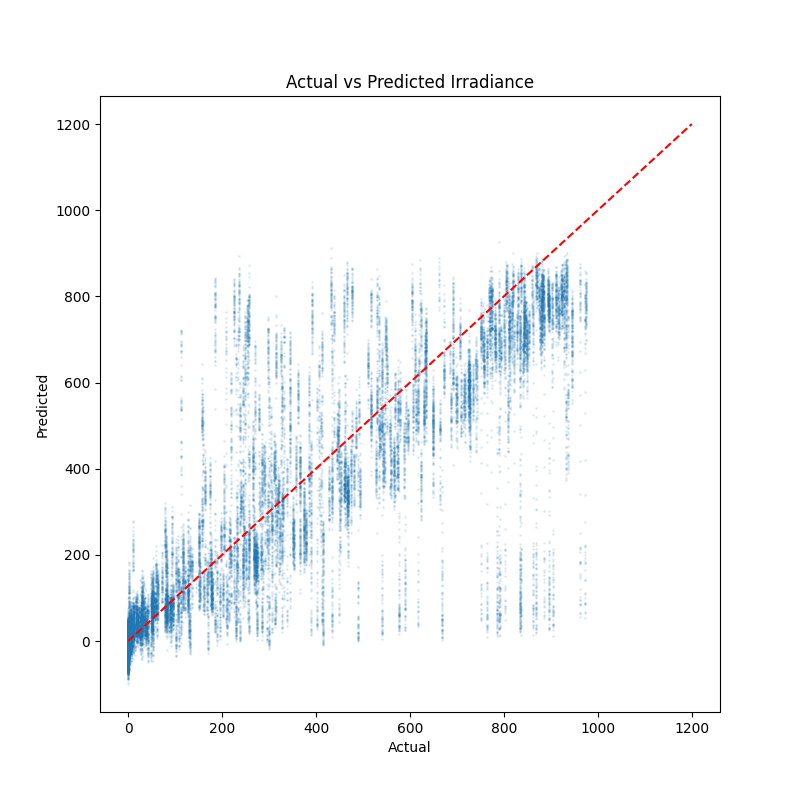
\includegraphics[width=0.6\textwidth]{artifacts/scatter_plot.png}
    \caption{Scatter Plot of Actual vs Predicted Irradiance.}
\end{figure}

\subsection{Quantitative Metrics}
The table below summarizes the performance metrics of our Hybrid BiLSTM-GBDT model.

\begin{table}[h]
    \centering
    \begin{tabular}{lccc}
        \toprule
        \textbf{Horizon} & \textbf{RMSE ($W/m^2$)} & \textbf{nRMSE (\%)} & \textbf{$R^2$ Score} \\
        \midrule
        24 Hours (1 Day) & 112.90 & 44.57\% & 0.8676 \\
        72 Hours (3 Days) & 125.91 & 49.83\% & 0.8351 \\
        168 Hours (7 Days) & 135.24 & 54.24\% & 0.8068 \\
        \bottomrule
    \end{tabular}
    \caption{Model Performance Metrics across different Forecast Horizons}
\end{table}

\subsection{Potential Application: Solar Power Output Estimation}
To demonstrate the practical utility of our irradiance forecasts, we explore a simplified application for estimating solar power generation. While complex physical models exist, the strong correlation between solar irradiance, ambient temperature, and photovoltaic (PV) energy output allows for the use of a simple Linear Regression model as an effective first-order approximation.

We propose a linear mapping function where the estimated power output $P_{est}$ is derived from the forecasted Global Horizontal Irradiance ($GHI_{pred}$) and ambient temperature ($T$):

\begin{equation}
    P_{est} = \beta_0 + \beta_1 \cdot GHI_{pred} + \beta_2 \cdot T + \epsilon
\end{equation}

Where:
\begin{itemize}
    \item $\beta_1$ represents the primary conversion efficiency coefficient related to irradiance.
    \item $\beta_2$ accounts for the temperature coefficient (typically negative, as efficiency drops with heat).
    \item $\beta_0$ is the intercept.
\end{itemize}

This lightweight add-on demonstrates how the medium-term irradiance forecasts generated by our hybrid model can be directly translated into actionable power generation metrics for grid operators, without the computational overhead of complex physical simulations. Preliminary analysis suggests that this linear approximation captures the bulk of the variance in power output, making it a viable tool for rapid scenario analysis and medium-term planning.

\section{Conclusion}
In this paper, we demonstrated the generalization capabilities of a hybrid BiLSTM-GBDT framework for medium-term solar irradiance forecasting. By validating the model across a diverse dataset of 22 BSRN stations, we showed that the approach remains robust across varying climatic conditions even without accounting for detailed meteorological data. The methodology highlights the effectiveness of using GBDT for structural feature extraction alongside BiLSTM for temporal modeling in data-constrained scenarios. Future work will focus on comparative analysis with other state-of-the-art models and the direct integration of power conversion modules.

\section{References}
\textit{[References to be added]}

\end{document}
